\documentclass[../../script.tex] {subfiles}
%! TEX root = ../../script.tex

\begin{document}
\section{Metric and Normed spaces}

\begin{defi}[Metric space]
    A metric space $(X, d)$ is an ordered pair consisting of a set $X$ and a mapping 
    \[
        d: X \times X \longrightarrow [0, \infty]
    \] 
    called metric. This mapping must fulfil the following conditions $\forall x, y, z \in X$:
    \begin{itemize}
        \item $d(x, y) \ge 0$ \text{ (Positivity)}
        \item $d(x, y) = 0 \iff x = y$ \text{ (Definedness)}
        \item $d(x, y) = d(y, x)$ \text{ (Symmetry)}
        \item $d(x, y) \le d(x, z) + d(z, y)$ \text{ (Triangle inequality)}
    \end{itemize}
\end{defi}

\begin{eg}
    \begin{enumerate}[(i)]
        \item Let $M$ be a set. Then 
        \[
            d(x, y) = \begin{cases}
                1, & x \ne y \\
                0, & \text{else}
            \end{cases}
        \]
        is called the discrete metric.

        \item Let $X$ be the set of edges of a graph.
        \begin{align*}
            d(x, y) := &\mbox{ Minimum amount of edges that have} \\
            &\mbox{ to be passed to get from } x \mbox{ to } y
        \end{align*}
        
        \begin{center}
            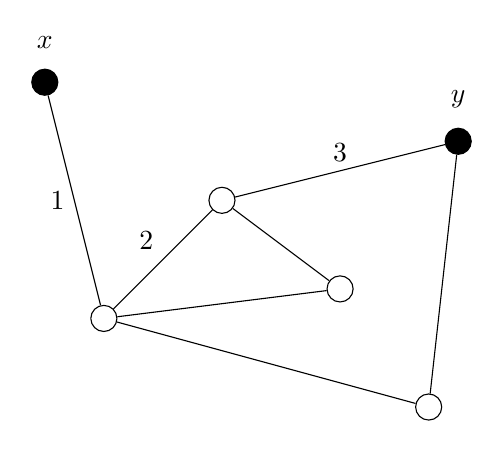
\begin{tikzpicture}[scale=0.75]
                \node[shape=circle, draw=black, fill=black] (A) at (0, 0) {};
                \node[shape=circle, draw=black] (B) at (1, -4) {};
                \node[shape=circle, draw=black] (C) at (3, -2) {};
                \node[shape=circle, draw=black] (D) at (5, -3.5) {};
                \node[shape=circle, draw=black] (E) at (6.5, -5.5) {};
                \node[shape=circle, draw=black, fill=black] (F) at (7, -1) {};

                \path [-] (A) edge node[left] {$1$} (B);
                \path [-] (B) edge node[above left] {$2$} (C);
                \path [-] (B) edge (D);
                \path [-] (B) edge (E);
                \path [-] (C) edge (D);
                \path [-] (C) edge node[above] {$3$} (F);
                \path [-] (E) edge (F);

                \node[above=0.3cm] at (A) {$x$};
                \node[above=0.3cm] at (F) {$y$};
            \end{tikzpicture}
        \end{center}

        \item Let $X$ be the surface of a sphere.
        \[
            d(x, y) := \text{"Bee line"}
        \]

        \item Let $X$ be the set of points of the European street network.
        \[
            d(x, y) := \text{ Shortest route along this network}
        \]

        \item Let $(X, d_X)$, $(Y, d_Y)$ be metric spaces. Then 
        \[
            d_{X \times Y}((x_1, y_1), (x_2, y_2)) := d_X(x_1, x_2) + d_Y(y_1, y_2)
        \]
        defines a metric on $X \times Y$.
    \end{enumerate}
\end{eg}

\begin{defi}[Normed space]
    $(V, \dnorm)$ is said to be a normed space if $V$ is a vector space and 
    \[
        \dnorm: V \longrightarrow [0, \infty)
    \]
    is a mapping (called norm) with the following properties
    \begin{itemize}
        \item $\norm{x} \ge 0$ (Positivity)
        \item $\norm{x} = 0 \iff x = 0$ (Definedness)
        \item $\norm{\lambda x} = |\lambda|\norm{x}$ 
        \item $\norm{x + y} \le \norm{x} + \norm{y}$ (Triangle inequality)
    \end{itemize}
    To every norm belongs a unique induced metric
    \[
        d(x, y) = \norm{x - y}
    \]
\end{defi}

\begin{eg}[$\realn^n$ with Euclidian norm]
    \begin{align*}
        \dnorm: \realn^n &\longrightarrow [0, \infty) \\
        (x_1, x_2, \cdots, x_n) &\longmapsto \sqrt{x_1^2 + x_2^2 + \cdots + x_n^2}
    \end{align*}
    Then $(\realn^n, \dnorm)$ is a normed space.
\end{eg}

\begin{eg}
    \begin{enumerate}[(i)]
        \item $(x_1, x_2, \cdots, x_n) \mapsto |x_1| + |x_2| + \cdots + |x_n|$ is also a norm on $\realn^n$.
        \item On
        \[
            V = \set[f \text{ continuous}]{f: [0, 1] \longrightarrow \realn}
        \]
        we can define the supremum norm 
        \[
            \supnorm{f} = \sup \set[{x \in [0, 1]}]{|f(x)|}
        \]
        \item We can define sequence spaces as 
        \[
            \ell^p = \set[\series{n} |x_n|^p < \infty]{\anyseqdef{\cmpln^n}}
        \]
        with the norm 
        \[
            \norm{(x_n)}_p := \sqrt{\series{n} |x_n|^2}
        \]
        A special space is $\ell^2$, called Hilbert space
    \end{enumerate}
\end{eg}

\begin{rem}
    The Minkowski metric is not a metric in this sense.
\end{rem}

\begin{defi}[Balls and Boundedness]
    Let $\metric$ be a metric space, and $x \in X, r > 0$. We then define 
    \begin{align*}
        \Oball(x) = \set[d(x, y) < r]{y \in X} && \text{Open ball} \\
        \Cball(x) = \set[d(x, y) \le r]{y \in X} && \text{Closed ball}
    \end{align*}
    A subset $M \subset X$ is called bounded if
    \[
        \exists x \in X, r > 0: ~~M \subset \Oball(x)
    \]
\end{defi}
\end{document}